\documentclass{article}



\usepackage{arxiv}

\usepackage[utf8]{inputenc} % allow utf-8 input
\usepackage[T1]{fontenc}    % use 8-bit T1 fonts
\usepackage{hyperref}       % hyperlinks
\usepackage{url}            % simple URL typesetting
\usepackage{booktabs}       % professional-quality tables
\usepackage{amsfonts}       % blackboard math symbols
\usepackage{nicefrac}       % compact symbols for 1/2, etc.
\usepackage{microtype}      % microtypography
\usepackage{lipsum}		% Can be removed after putting your text content
\usepackage{graphicx}
\usepackage[square]{natbib}
\usepackage{doi}
\usepackage{parskip}
\usepackage{multirow}
\usepackage[table]{xcolor}
\usepackage{pdflscape}
\usepackage{longtable}

\title{A Review of Hollow Rotating Detonation Engines}

%\date{September 9, 1985}	% Here you can change the date presented in the paper title
%\date{} 					% Or removing it

\author{ \href{https://orcid.org/0000-0002-0831-3736}{
\includegraphics[scale=0.06]{orcid.pdf}\hspace{1mm}Reuben Hann}\\
%\thanks{Use footnote for providing further information about author (webpage, alternative address)---\emph{not} for acknowledging funding agencies.} \\
	School of Aerospace, Transport and Manufacturing\\
	Cranfield University\\
	Cranfield, MK43 0AL, UK \\
	\texttt{reuben.hann@cranfield.ac.uk} \\
	%% examples of more authors
	\And
	\href{https://orcid.org/0000-0002-2898-2056}{
\includegraphics[scale=0.06]{orcid.pdf}\hspace{1mm}Enric Grustan-Gutierrez} \\
	School of Aerospace, Transport and Manufacturing\\
	Cranfield University\\
	Cranfield, MK43 0AL, UK \\
	\texttt{e.grustan@cranfield.ac.uk} \\
	%% \AND
	%% Coauthor \\
	%% Affiliation \\
	%% Address \\
	%% \texttt{email} \\
	%% \And
	%% Coauthor \\
	%% Affiliation \\
	%% Address \\
	%% \texttt{email} \\
	%% \And
	%% Coauthor \\
	%% Affiliation \\
	%% Address \\
	%% \texttt{email} \\
}

% Uncomment to remove the date
%\date{}

% Uncomment to override  the `A preprint' in the header
\renewcommand{\headeright}{}
%\renewcommand{\undertitle}{Technical Report}
\renewcommand{\shorttitle}{Review of Hollow Rotating Detonation Engines}
%\textit{arXiv} 

%%% Add PDF metadata to help others organize their library
%%% Once the PDF is generated, you can check the metadata with
%%% $ pdfinfo template.pdf
\hypersetup{
pdftitle={A Review of Hollow RDEs},
pdfauthor={Reuben Hann},
}

\begin{document}
\maketitle

\begin{abstract}
The demands on chemical propulsion systems have never been greater. Pressures from climate change and more competitive satellite and space launch markets require that propulsion systems be more compact, efficient and cost-effective. One technology that could meet these aims is rotating detonation engines (RDEs). RDEs operate by continuously rotating a detonation wave around an annular or cylindrical (hollow) combustion chamber. The shockwave of the rotating detonation wave compresses the propellants beyond their initial conditions, improving the overall combustion system’s efficiency. The hollow RDE combustor design has reduced cooling requirements, steadier outflow and thrust compared to annular RDEs. As hollow RDEs are an important development in the RDE research field, this paper provides an overview of the current state of hollow RDE research such as the discovery of the wall-detached rotating detonation mode and development of flow-through RDEs and identifies research gaps and paths forward for further research, for example validating the emissions profiles of hollow RDEs, and investigating the use of annular RDE reduced-order mathematical models in hollow RDE research.
\end{abstract}


% keywords can be removed
\keywords{Hollow RDE \and Rotating Detonation \and Propulsion}


\section{Introduction}

Combustion has been one of humanity’s primary means of generating energy for thousands of years and increasingly so over the past 300 years. The burning of fossil fuels generates greenhouse gas emissions which significantly contribute towards climate change. To reduce emissions, two trends have been taking place. First, is to move away from combustion as a primary energy source and second is to improve the efficiency of combustion. One potential avenue for improving the efficiency of combustion is detonation.
\par

There are two forms of combustion, deflagration and detonation, primarily differentiated by the flame speed, the velocity a flame front expands in a mixture of fuel and oxidiser. Deflagration has subsonic flame speeds, typically 1-100 m/s, whereas detonation has supersonic flame speeds in the region of 1500-2500 m/s. The supersonic flame speed leads to the detonation wave comprising a leading shockwave and an attached combustion region behind it. This leading shockwave compresses the reactants before being burnt, allowing the combustion to occur at a higher pressure and temperature than if the reactants were deflagrated rather than detonated, improving the combustion system efficiency\cite{Zeldovich2006}. If fully realised, this could allow there to be a gain in total pressure over the combustor, as opposed to a pressure loss typically found in jet and rocket engine combustors. Using detonation in combustion engines in the form of rotating detonation has so far experimentally shown a 5-7\% reduction in specific fuel consumption in gas turbines and a 6-8\% higher specific impulse in rocket engines though no total pressure gain over the combustor has yet been achieved \cite{1Anand2019}.
\par

Though detonation comes with improvements in efficiency, current jet and rocket engine combustion chambers are designed to avoid and quench it, as detonation can cause damage to the combustor and potential failure of continuous combustion. The higher flame speeds, combustion temperatures and pressure gradients caused by the detonation wave all contribute to this. Detonation is also not practical in internal combustion engines (ICEs). Often known as knocking or pinging in ICEs, detonation can damage parts of the engine and as such is actively avoided. As current combustor designs are incompatible with detonation, alternative approaches have been developed. The two primary approaches to implementing detonation-based combustion are pulse detonation engines (PDEs) and rotating detonation engines (RDEs).
\par

Similar to a pulsejet engine, PDEs operate on the cycle: the chamber is filled propellants, the chamber is sealed off at the inlet, the propellants are deflagrated and the burnt products ejected from the chamber to generate thrust. This cycle is repeated at a frequency from around 5-200Hz \cite{Pandey2016}. PDEs adopt this cycle but use detonation as opposed to deflagration, increasing the efficiency. This implementation of detonation propulsion has the benefit of being mechanically simple, as it can operate without the need for a compressor but produce periodic thrust as opposed to continuous thrust by a jet or rocket engine. This can cause vibration issues and possibly structural issues, though this is an issue that affects pulsejets as well.  
\par

RDEs solve the issue of periodic combustion by allowing for continuous detonation by adding directionality to the detonation wave. By injecting a detonation wave tangentially into an annular or cylindrical combustion chamber as seen in Figure \ref{Fig.1}, the detonation wave will continuously rotate around the inside wall of the chamber. This process is then sustained by injecting reactants along the axis of the combustion chamber in an annular injection area. The combusted products are then ejected out of the other end along the axis of the chamber into a turbine or a nozzle to generate thrust. 
\par

\begin{figure}
\centering
\includegraphics[scale=0.25]{HRDE_dia_labeledcrop.png}
\caption{Diagram of a hollow RDE with 2 co-rotating detonation waves. The numbers describe each of the stages of the flow in an RDE.}\label{Fig.1}
\end{figure}

RDEs are typically classified by their combustion chamber geometry, being either annular or cylindrical. The cylindrical combustion chamber geometry is referred to as a hollow RDE. This is because the annular RDE geometry has been the primary design for decades, being first explored in the 1960’s \cite{Nicholls1966}. An annular combustion chamber is made of two cylinders, one inside the other and the combustion occurs in the gap between the two. When the hollow RDE design first started being explored in early 2011 \cite{Shao2011}, the geometry was conceived by removing the inner cylinder, therefore creating a hollow chamber. It was discovered that the inner cylinder was not necessary to sustain a rotating detonation wave and that the inner cylinder induced losses on the detonation wave due to heat transfer and wall effects \cite{Shao2011}. The improvement in detonation performance is significant as seen in the detonation wave velocities where annular RDEs typically have 60-80\% and hollow RDEs have 80-100\% CJ velocities \cite{Liu2021}. The CJ velocity refers to the Chapman Jouguet velocity, the calculated idealised detonation velocity. This improvement in detonation performance comes with a simpler engine geometry, reduced cooling requirements and similar operating characteristics. These benefits though do potentially come with several downsides, such as the larger chamber volume potentially being harder to initiate than annular designs, and the increased combustion residence time in the central region of the chamber. This can cause parasitic deflagration where propellants are deflagrated rather than detonated decreasing the efficiency of the combustor. Furthermore, the knowledge gaps in this research field are broad, because it is a recent and niche research field, with only a small number of teams researching this technology in the US \cite{Wiggins2023}, China \cite{Xue2022} and Japan \cite{Nakata2022}. These research gaps provide ample opportunities to explore and further develop this technology.
\par

Therefore, in this paper, the current state of the hollow RDE research field is categorised, the research gaps are identified and further avenues for research are suggested. 

\section{Methodology}

As of June 2023, there have been around 60 publications total, both conference papers and journal publications researching hollow RDEs. These publications were found through keyword searching and searching through citations in these papers. The scientific paper search engines that were used were Google Scholar and Elsevier and the primary keywords used to search for papers were: “RDE”, “rotating detonation”, “hollow”, and “centerless”, these being the most common terms used within hollow RDE research. Additionally, summary papers on the whole RDE research field \cite{1Anand2019,Xie2020}, were used to find publications through their citations. Though these summary papers primarily focus on annular RDEs, they do briefly cover hollow RDEs and provide a solid starting point for researching the larger RDE research field. The resulting papers gathered were then filtered for duplicate papers and papers not studying hollow RDEs and categorised based on the countries the research was conducted in, if the research was numerical or experimental work, and the propellant types studied. 


\section{Discussion}\label{sec:Discussion}
\subsection{Annular and Hollow RDEs}\label{subsecAnnular and Hollow RDEs}

The removal of the inner wall of a rotating detonation combustor, thereby converting an annular RDE into a hollow, or centre-bodiless RDE introduces meaningful changes to the performance, design and implementation of a rotating detonation combustor. A core example of this is shown by the implementation of a nozzle onto each of the combustor geometries, with converging-diverging nozzles easily integrated onto the circular cross-section of a hollow RDE, and the annular cross-section aerospike nozzle fitting the the annular geometry of an annular RDE \cite{1Anand2019}.
\par

Annular RDEs have been shown to be susceptible to thrust stability issues at higher mass flow rates and atmospheric ambient pressures such that there are large errors when using traditional steady-state thrust equations and can suffer from significant reverse flow into the nozzle which degrades the thrust stability \cite{Sun2018}. The considerably larger combustion chamber volumes of hollow RDEs can counter act this, as the hollow RDE’s large centre region acts to dampen the variations in exit flow and pressure caused by the transient nature of using rotating detonation \cite{Sun2019}. The larger chamber volume also provides potential challenges with longer residence times and parasitic deflagration occurring in the centre region \cite{Tang2015} which could decrease the performance of the engine, with propellants being deflagrated rather than detonated and NOx formation in the case of air being the oxidiser. 
\par

Though on the face of it, all forms of detonation combustion appears to face several challenges with NOx emissions as a result of the  higher flame temperatures and reduced flammability limits of detonation as opposed to deflagration. These counteract the traditional NOx mitigation strategies of running leaner mixtures and reducing flame temperatures. Additionally, the longer residence times of hollow RDEs add to these apparent challenges increasing the time spent at higher temperatures, potentially increasing NOx emissions. However, though there is limited data available on RDE emissions more generally, the hollow RDE NOx emissions data available is promising, with emissions of around 10 ppm(v) NOx at 15\% O2, corresponding to approximately 15 mg/MJ NOx emissions whilst using hydrogen \cite{Stoddard2017}. This is within the EU Clean Hydrogen Partnership NOx targets for 2030 for state-of-the-art hydrogen gas turbines (<25 ppm(v) at 15\%O2, and <24 mg/MJ NOx). Furthermore, this result was achieved with a laboratory hollow RDE, which has not been designed or optimised to minimise NOx emissions. 
\par

\begin{figure}
\centering
\includegraphics[scale=0.75]{Hollow_RDE_Share.png}
\caption{Number of RDE and hollow RDE publications and each year since 2010.}\label{Fig.2}
\end{figure}


The results are also comparable to annular RDEs NOx emissions at approximately 11 NOx ppm(v) at 15\% O2 \cite{Ferguson2020}. This suggests that the residence times are similar, for both hollow and annular RDEs at around 0.2ms \cite{Anand2019} for at least the current size of RDEs being researched, <150mm diameter. Numerical research has suggested further methods of reducing NOx in RDEs such as increasing the mass flow rate and maximising the strength of the detonation wave, thereby increasing the pressure and temperature gradients, resulting in a more rapid expansion after the detonation wave with the primary aim of minimising the residence time, regardless of the combustion temperatures to minimise NOx emissions. However additional strategies to further reduce the residence times in hollow RDEs such as flow-through hollow RDEs, are still in their infancy and require further research to obtain stable operation \cite{Wiggins2023}. However, the reliability and repeatability of the readings can be reasonably questioned given the unsteady nature of RDEs and exhaust products. Further work is needed to develop more adequate research methodologies for transient combustor emissions to validate current findings \cite{Anand2019}.
\par

Annular RDEs have been around for considerably longer than hollow RDEs, though research into RDEs only recently gained pace since 2010 with an exponential growth in the number of publications about RDEs ever since \cite{Wang2020}. This research into annular RDEs has yielded significant results, as shown by NASA developing a reusable 10,000lbf (44.5kN) annular RDE rocket engine and testing in 2022 \cite{Osorio2023}. Hollow RDEs on the other hand only started being researched in the latter part of the 2010s \cite{Stoddard2015} and have been around 1.7-8.6\% of the total research into RDEs since their conception as shown by Figure \ref{Fig.2}. Research into hollow RDEs is growing as shown by Figure \ref{Fig.3} but is approximately at least a decade or twop behind annular RDEs in terms of research and development. 
\par

Hollow RDEs show promise, having a simple, more easily manufactured design, and cooling system compared to annular RDEs, whilst still retaining the specific impulse increases and specific fuel consumption decreases of rotating detonation compared to deflagration combustors \cite{1Anand2019}. In addition to hollow RDE’s low NOx emissions using hydrogen \cite{Stoddard2017} and more compact combustors \cite{Ishihara2023} compared to deflagration combustors, hollow RDEs show promising results for integration into future propulsion and energy generation systems.
\par

\begin{figure}
\centering
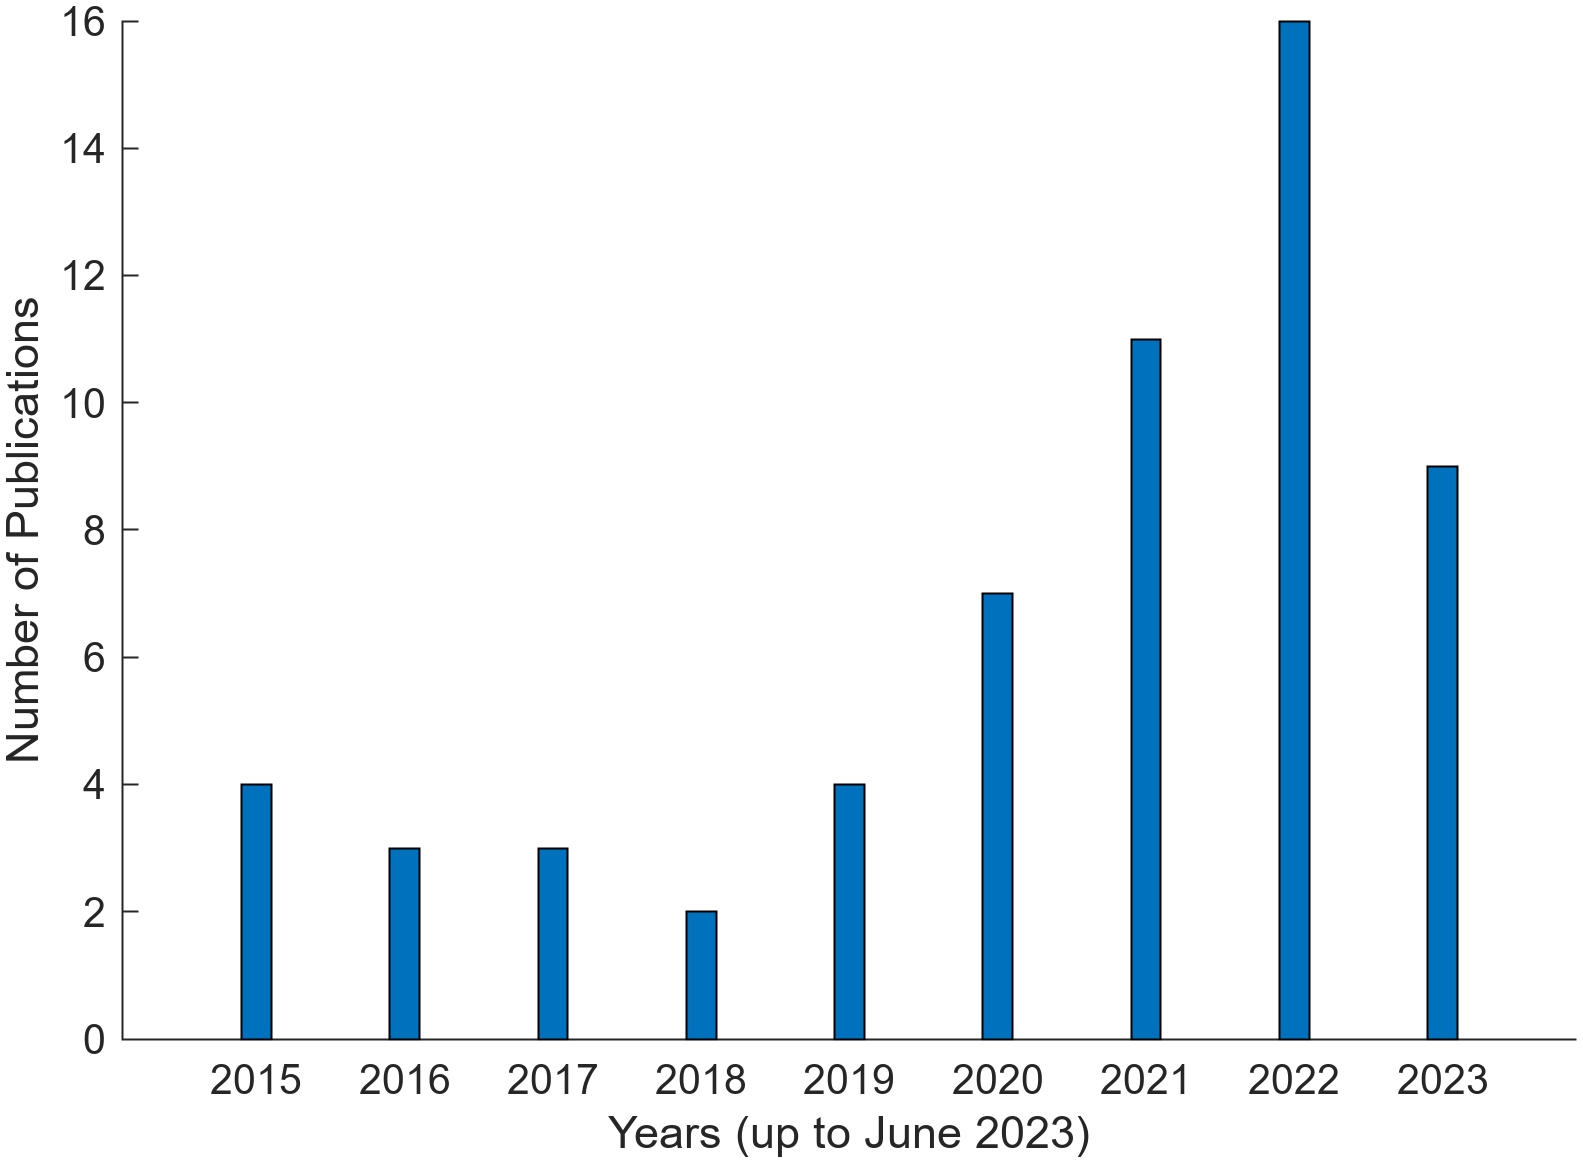
\includegraphics[scale=0.75]{HRDEpubsovertime.png}
\caption{Number of hollow RDE publications each year up to mid 2023.}\label{Fig.3}
\end{figure}

\subsection{Hollow RDE Research Field}

Within the hollow RDE research field, so far China has contributed the largest number of research papers with up almost 60\% of publications as seen in Figure \ref{Fig.4}. US-based researchers have published approximately a quarter of publications, with Japan-based researchers publishing half that of US-based researchers.  Across the hollow RDE research field, there has been very little direct collaboration between researchers based in different countries. So far there are only two studies where this has taken place, one between China and Japan \cite{Xia2018} and one between the US and Japan \cite{Yokoo2021}. No direct cooperation between researchers based in China and the US has occurred so far. This is possibly due to most hollow RDE research in the US either being funded by or being conducted by military-related sources. In contrast, all hollow RDE research in Japan has been funded by civilian agencies, whereas hollow RDE research in China has been a mixture between military and civilian. Given the small size of the research field and likely national security concerns given that RDEs have applications in space propulsion, hypersonics, rocket and aircraft propulsion, cooperation is likely to be limited for the foreseeable future between different researchers and research groups in different countries.

\begin{figure}
\centering
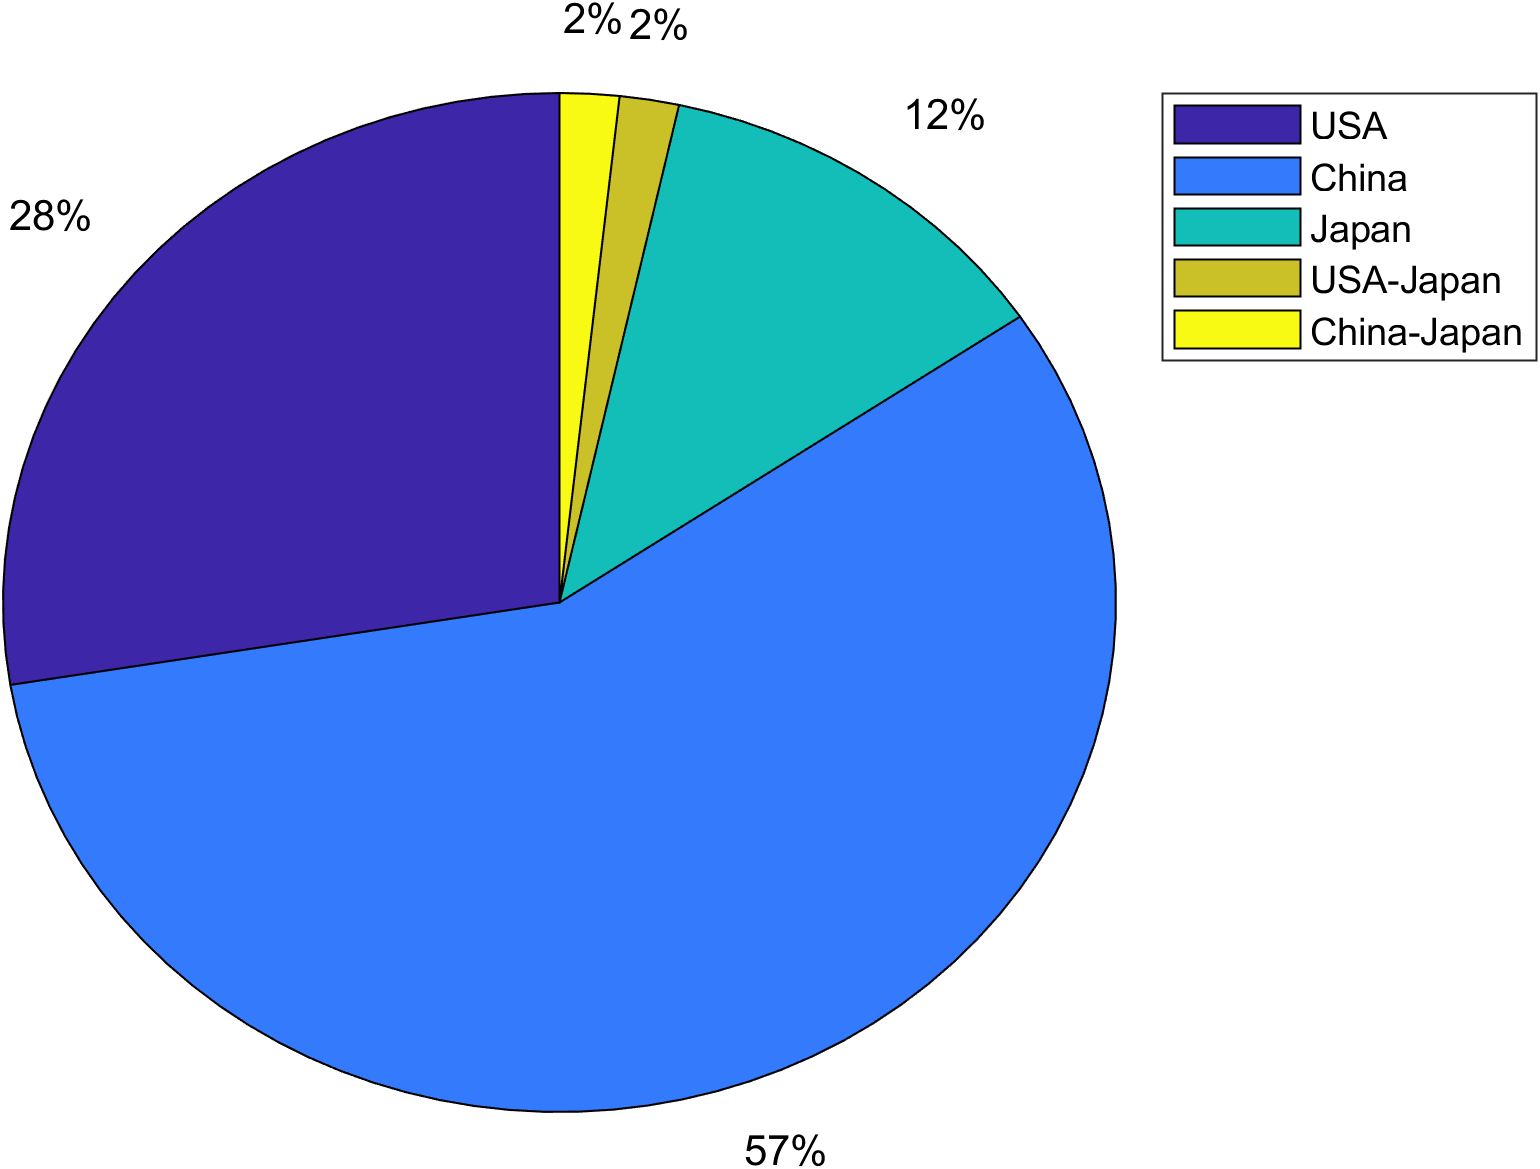
\includegraphics[scale=0.75]{HRDEpubcountry.png}
\caption{Distribution of Hollow RDE research by country.}\label{Fig.4}
\end{figure}

\subsection{Experimental Performance}

A core aspect to the performance of a hollow RDE are the propellants used. A wide range of propellant combinations have been tested as shown in Figure \ref{Fig.5}. As a general rule, the more chemically simple the propellants, the easier it is to detonate and the lower the ignition energy \cite{Shepherd2002}. Given that both numerical and experimental testing are essential to research into hollow RDEs, this also provides the benefit of the propellants being computationally easier to simulate, as chemically simpler propellant combinations typically have smaller reaction mechanisms \cite{CERFACS}. This has lead to the primary use of chemically simple propellants as opposed to large complex hydrocarbons within hollow RDE research as seen in Figure \ref{Fig.5}.
\par

Propellant choice not only has ignition and numerical simulation concerns but directly impacts all aspects of an RDE as seen in Figure \ref{Fig.6} due to RDE design being incredibly coupled. Hydrogen is the most common fuel used across the hollow RDE research field with 51\% of publications using the fuel. As hydrogen does not contain carbon, it produces no soot or carbon dioxide which makes it attractive as a fuel in the move towards net-zero. Hydrogen’s other properties such as its low initiation energy, wide detonability range and as a gaseous propellant, can be easily pressure fed into the combustion chamber have led it to be the main fuel used in hollow RDE research. In addition, though its density is low especially compared to hydrocarbon fuels, its high oxidiser-to-fuel ratio can help offset the required volumetric flow rate of hydrogen.
\par

\begin{figure}
\centering
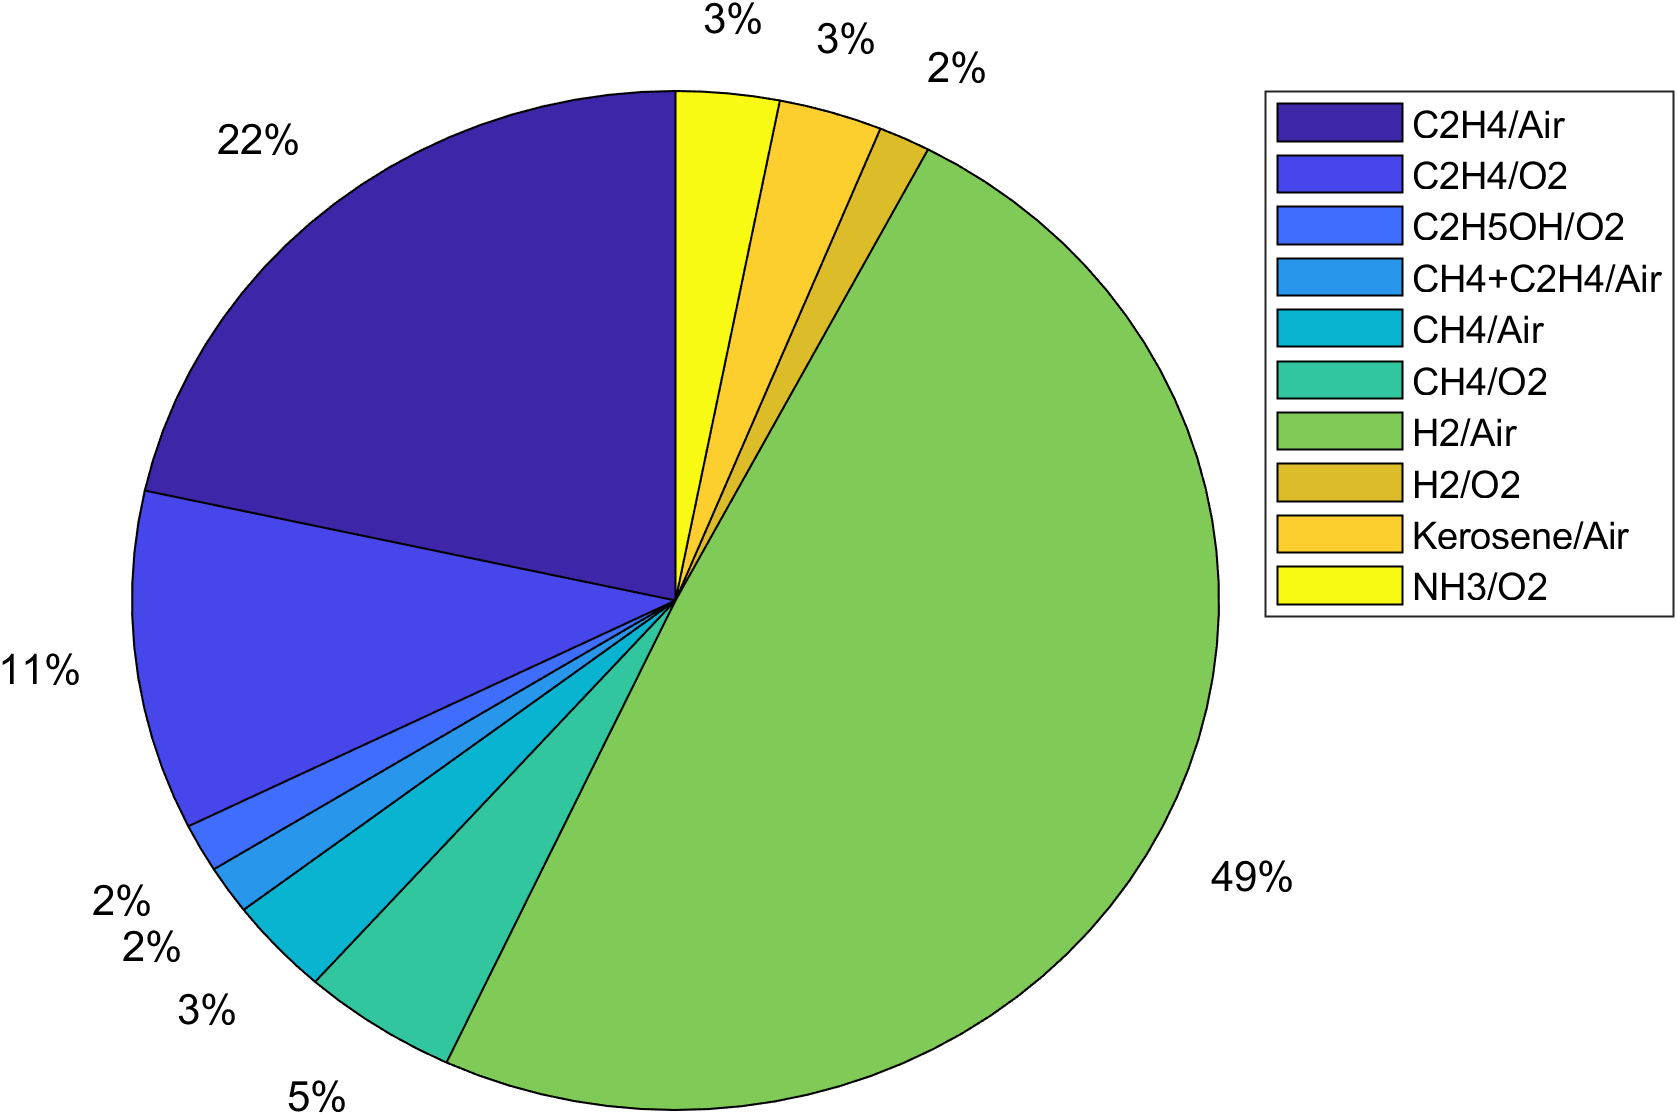
\includegraphics[scale=0.75]{HRDEfuelspie.png}
\caption{Percentage of publications using each particular propellant combination.}\label{Fig.5}
\end{figure}

Ethylene is the secondary choice as a fuel for research into hollow RDEs, as a hydrocarbon it is denser than hydrogen and less prone to leaks. It is also safer and less easy to detonate than acetylene, another hydrocarbon which is also cheap and widely available. Acetylene is one of the easiest to detonate fuels especially compared to butane or propane, but has been considered too easy to detonate for safe and easy use in detonation engines. Methane is a good alternative to ethylene, having similar properties and benefits, but has been used less frequently. Ammonia similar to hydrogen has potential as a net-zero fuel by not containing carbon, but can be hard to detonate \cite{Huang2022,1Huang2022} and can be more expensive than pure hydrogen. Though Ammonia liquefies at much lower pressures and temperatures and can be stored for a long time, unlike hydrogen. Kerosene \cite{Xue2022} and ethanol \cite{1ISHIHARA2023} have been tested proving that two-phase liquid propellants can be used with hollow RDEs successfully, but further research is needed to better understand the impact of two-phase flow on hollow RDE detonation and engine performance. 
\par

Experimental thrust and specific impulse is currently very limited for hollow RDEs with very few papers published \cite{Yokoo2020,Goto2022,Nakata2022,Yokoo2021,Ishihara2023,1ISHIHARA2023,Lin2020}. Whereas experimental detonation performance data collection such as detonation velocities and modes has been the core focus of research on hollow RDEs so far as seen in Table \ref{table1}. The higher \%CJ velocities found in hollow RDEs has been recreated across a wide range of reactants, for example, an Ammonia and Oxygen hollow RDE achieving around 75\% CJ velocity  \cite{Huang2022}, Kerosene and Air reaching around 90\% CJ velocity\cite{Xue2022}, or repeatedly reaching 100\% CJ velocity when using Hydrogen and Air \cite{Wang2019}.
\par
% https://coolors.co/palette/d8e2dc-ffe5d9-ffcad4-f4acb7-9d8189
\begin{table}
	\caption{Number of Experimental Publications with Performance Data (Detonation data e.g., detonation velocity, frequency etc..., Engine data e.g., thrust, specific impulse, etc...)}
	\centering
	\begin{tabular}{lllll}
		\toprule
		\multirow{1}{*}{} & \multicolumn{2}{c}{Oxygen} & \multicolumn{2}{c}{Air} \\
		\cmidrule(r){2-5}
		Fuel     & Detonation data    & Engine data & Detonation data & Engine data\\
		\midrule
		Hydrogen    & \cellcolor[HTML]{FFCAD4} 1 & \cellcolor[HTML]{F4ACB7} 0 & \cellcolor[HTML]{D8E2DC} 32 & \cellcolor[HTML]{FFCAD4} 1 \\
		Ammonia     & \cellcolor[HTML]{FFCAD4} 2 & \cellcolor[HTML]{F4ACB7} 0 & \cellcolor[HTML]{F4ACB7} 0 & \cellcolor[HTML]{F4ACB7} 0 \\
		Methane     & \cellcolor[HTML]{FFCAD4} 3 & \cellcolor[HTML]{F4ACB7} 0 & \cellcolor[HTML]{FFCAD4} 2 & \cellcolor[HTML]{F4ACB7} 0 \\
        Ethylene    & \cellcolor[HTML]{D8E2DC} 14 & \cellcolor[HTML]{FFE5D9} 5 & \cellcolor[HTML]{D8E2DC} 15 & \cellcolor[HTML]{F4ACB7} 0 \\
        Ethanol     & \cellcolor[HTML]{FFCAD4} 1 & \cellcolor[HTML]{FFCAD4} 1 & \cellcolor[HTML]{F4ACB7} 0 & \cellcolor[HTML]{F4ACB7} 0 \\
        Kerosene    & \cellcolor[HTML]{F4ACB7} 0 & \cellcolor[HTML]{F4ACB7} 0 & \cellcolor[HTML]{FFCAD4} 2 & \cellcolor[HTML]{F4ACB7} 0 \\
		\bottomrule
	\end{tabular}
	\label{table1}
\end{table}

\subsection{Hollow RDE propagation Influences}\label{Hollow RDE propagation Influences}

\begin{figure}
\centering
\includegraphics[scale=0.5]{Hollow RDE Modification of Fig 4.1. from Review on the Rotating Detonation Engine and It’s Typical Problems.png}
\caption{Interactions between the different aspects of rotating detonation and RDE Design. An expanded version of Figure 4.1. in Review on the Rotating Detonation Engine and Its Typical Problems by Q. Xie et al., (2020) \cite{Xie2020} }\label{Fig.6}
\end{figure}

RDEs exhibit highly coupled dynamics, where the design, geometry and operating conditions collectively influence the performance and stability of the rotating detonation wave, as shown in Figure \ref{Fig.6}. At ignition, the predetonator injects the nascent detonation wave tangent to the chamber, with the directionality to drive rotating detonation \cite{Zhang2017}. Core to sustaining the rotating detonation wave is the concept of mixture efficacy. This term encapsulates how optimal the post-injection propellant mixture is at sustaining the rotating detonation wave, considering both the quality of the post-injection mixture and its availability. 

Mixture efficacy is driven by the choice of propellants, injector and nozzle design and exit conditions. The choice of propellants along with the detonation mode, dictates the detonation velocity and, consequently, the period of the detonation wave. The design of the injector, also influences mixture efficacy which determines the mixing efficiency and the homogeneity of the mixture \cite{Gaillard2015} and the nozzle design and exit conditions are critical for the efficient extraction of burnt products. Suboptimal design of the nozzle can lead to burn products recirculating, adversely affecting mixing efficacy \cite{Wang2019}.
An additional factor is the interaction between the injection process and the internal flow within the combustion chamber. If the injectors are unchoked, the rotating detonation wave and reflected shockwaves can induce pressure oscillations in the propellant feed system, potentially leading to instabilities in the injection process and disrupting the rotating detonation wave \cite{Sada2022}. Minimising sudden changes in geometry and careful positioning of the predetonator and nozzle can mitigate the impact of reflected waves, \cite{Wang2019,1Zhang2021}.

A fundamental design parameter of an RDE is the combustion chamber diameter, which typically corresponds to the radius at which the detonation wave rotates \cite{1Huang2023}. This parameter, in conjunction with the number of detonation waves and the detonation velocity, related to the detonation mode, determines the engine’s operating frequency and the period of the detonation wave. The detonation mode itself can influence the rotating detonation process. Altering the mode, the number of detonation waves, and their strength by modulating the mass flow rate, though to a lesser degree by altering the other factors \cite{Xie2018}, can affect the stability of the rotating detonation wave. While the most stable modes in hollow RDEs usually feature one to two detonation waves \cite{1Zhang2021}, operating with more waves increases the risk of instability. More waves reduce detonation wave strength and speeds of the waves, impacting the timing balance of propellant injection, consumption, and ejection. These highly coupled mechanisms combine and interact to form the rotating detonation phenomenon, balancing the core design variable of the injector, nozzle and combustion chamber design along with the propellant choice, stable rotating detonation can occur. 

\subsection{Detonation Dynamics}

The detonation dynamics of hollow RDEs have been broadly studied and resemble annular RDEs \cite{Schwer2020,Schwer2021}. Though other factors can influence stability of the detonation wave in RDEs, as the mass flow rate has the largest influence, the other factors are disregarded \cite{Xie2018}.
\par

After initiation using a predetonator, if successful, the injected detonation wave transitions into rotating detonation which will have a specific detonation mode. At a too low mass flow rate, the rotating detonation wave will fall back to deflagration but continue rotating. A rotating deflagration wave is defined by the lack of a shock wave \cite{Huang2019,1Huang2019}. At a higher mass flow rate, the injected detonation wave can fall between deflagration and detonation, this critical mode is called Sawtooth-wave mode. In Sawtooth-wave mode pressure measurements, there is no typical detonation pressure plot with an exponential pressure drop-off from the pressure peak. The pressure plot resembles a sawtooth wave with a linear pressure drop-off  \cite{Huang2019,1Huang2019,Peng2022}. Though the Sawtooth wave mode peak pressures and wave speeds are higher than rotating deflagration, they are lower than a rotating detonation wave. Increasing the mass flow rate further strengthens the wave to form a singular rotating detonation wave. In most RDEs researched thus far, this is the most stable operating mode for rotating detonation \cite{Huang2019,1Huang2019}. 
\par

Further increasing the mass flow rate intensifies the detonation wave such that the detonation wave’s shockwave gets reflected off the converging section of the nozzle, causing the two pressure peak signals in the single detonation wave pressure reading \cite{Huang2019,1Huang2019}. As such this mode is called Two Dominant Peak One wave mode (TDPO). An additional mass flow rate increase results in the single detonation wave splitting into two co-rotating detonation waves. Rotating detonation waves will split, extinguish themselves, or merge to reach a balance between the population of rotating detonation waves, their rate of consumption of the propellants, the rate of injection of propellants and how well waste products are removed so long as it is within a stable operating regime \cite{1Rong2022,Smith2021}. This results in the increase in the number of co-rotating detonation waves as the mass flow rate increases. Each increase in the number of co-rotating detonation waves decreases the strength, pressure rise and detonation velocity of each wave. Increasing the number of detonation waves up to a point causes the velocity of the co-rotating waves to decrease below the speed of sound, causing the rotating detonation to fail, reverting the combustion from detonation to deflagration or blow-off \cite{Andrus2017}. As most research has occurred using low mass flow rates, and small chamber sizes, there have been few experimental examples of >2 detonation co-rotating detonation waves in hollow RDEs [41] as such further research is needed to explore this range of operation modes.
\par

Since rotating detonation has similar characteristics to high-frequency tangential combustion instabilities, rotating detonation dynamics and modes especially in hollow RDEs are of high interest. Hollow RDE operating frequencies are within 5\% of 1T+1L mode combustion instability \cite{Zhang2021}. As hollow RDEs have a much more similar combustor geometry to that of a rocket, high-frequency tangential combustion instabilities may be unintended rotating detonation waves. To date, no single study in the hollow RDE research field has gone in-depth and systematically validated that high-frequency combustion instabilities are a form of rotating detonation, but evidence suggests a strong connection between the two. Another detonation phenomenon that is of interest is counter-rotating detonation waves. Though this mode in hollow RDEs has only been explored numerically \cite{1Rong2022,2Rong2022}, this mode of operation has been widely observed in annular RDEs \cite{Zhao2020}. This mode of operation is highly unstable, and complex and requires further investigation in experimental experiments to prevent this mode \cite{2Rong2022}.

\subsection{CFD and Numerical Modelling}

The rise in research into RDEs has grown with the rise over the last 20 years of accessible and high-performance computing power. With this computing power, Computational Fluid Dynamics (CFD) has become a viable way to test concepts and designs and help reduce the amount of time and cost of experimental testing. CFD allowed the simulation of RDEs. Given the high mesh refinement with cell sizes (approximately 0.5mm to 0.1mm) \cite{Nakata2022}, small step sizes (around 1e-7s to 1e-9s), and often large reaction mechanisms required to accurately simulate rotating detonation, the computing power to conduct such research was only commercially available over the past 15-20 years.
\par

CFD simulations were used to test the initial concepts behind removing the inner wall of annular RDEs to create the first hollow RDE concepts in 2011 and 2015 \cite{Shao2011,Tang2015,1Stoddard2015}. As hollow RDEs greatly increase the volume of the combustion chamber, the computational cost of simulating hollow RDEs is vastly greater than annular RDEs. This has hindered the accessibility and accuracy of the simulations conducted as numerical research is being relegated to heavily simplified CFD approaches and models of hollow RDEs to reduce computational costs. Most simulations have been conducted using Euler/Inviscid models \cite{Xia2018,Tang2015,Yao2017} ignoring turbulence within the domain. Whilst this simplifies the complex simulations, this approach can severely miss the important effect boundary layers can have in RDEs, as seen by Japanese researchers who build a reduced order model to predict the boundary layer growth in their small scale (20mm diameter) hollow RDEs \cite{Nakata2022,Yokoo2020}. They found this boundary layer could choke the outflow of their small RDE without a nozzle. \cite{Nakata2022,Yokoo2020}. A few hollow RDE studies have used Reynolds-Averaged Navier-Stokes (RANS) approaches \cite{Sun2019}, but none so far have used Large Eddy Simulation (LES) viscous models, creating a gap in the research field given the highly unsteady flow in hollow RDEs.
\par

As discussed earlier in this section, reduced order models for hollow RDEs have been developed, though have not been widely adopted or referenced past their original publications. A quasi-steady 1D model of a hollow RDE has been developed and tested with small-diameter hollow RDEs and found to reasonably match their experimental results for the axial pressure distribution along the combustion chamber \cite{Nakata2022} this model was adapted to predict the growth of the boundary layer and choking of the outflow via the boundary layer in a small hollow RDE without a nozzle \cite{Yokoo2021}. Finally, a reduced order model was used to model the thermal transfer for a novel injector wall injected propellants design to model the temperature reduction by injecting propellants from the wall.
\par

\subsection{Measurement Approaches}

The primary measurement techniques of hollow RDEs are using pressure Capillary Tube Average Pressure (CTAP) sensors which use capillary tubes to dampen pressure waves and keep pressure sensors safe from the engine heat. These allow high-speed pressure measurements to be taken and can record the distinctive shape of the detonation wave over time as it passes over. This being a sharp disconnected vertical jump in pressure to the detonation pressure and a rapid exponential decrease in pressure back to the combustion chamber pressure. By observing the pressure wave, we can measure the velocity of the wave by measuring the peak-to-peak time. The produced pressure-over-time and velocity data allows the detonation mode of the engine to be found. Using a second pressure sensor placed in a different radial position can allow measurement of the number of rotating detonation waves and stability by comparing the detonation wave timings between the two or more sensors. If the time lag between detonation wave peaks is stable, then the detonation is in a stable detonation operating mode \cite{Betancourt2021}.  Spectral proper orthogonal decomposition (SPOD) analysis has been conducted on CTAP pressure measurements to further decompose the modes of operation \cite{Betancourt2021}.
\par

CTAP sensors though predominantly used to measure the detonation performance of the engine are an invasive approach requiring tapping of the engine and only provide a single point to measure and record data. Non-invasive measurement techniques have been an area of interest in the research field to provide alternative methods of analysing hollow RDEs. Strain gauges have been used for measuring the operating frequency by measuring the vibrations of the engine but have been unable to measure the operating mode or detonation velocity accurately \cite{Pritschau2022}. By using high-speed cameras, OH or CO chemiluminescence imaging, we can record the rotating detonation wave through optical windows \cite{Peng2020}, by building the entire combustion chamber out of transparent high-temperature quartz glass \cite{Wang2019} and by looking straight down the bore of the chamber \cite{Gaetano2022}. The chemiluminescence measurements create tomographic imaging of the detonation wave structure \cite{Gaetano2021}. High-speed imaging of the combustion chamber provides significant challenges, such as optical windows providing a stress-fracture point due to the different thermal expansion coefficients between the optical port and chamber wall materials. Otherwise constructing the chamber out of high-temperature quartz glass or other high-temperature optical materials is limited by the cost, strength and short lifespan of these materials in a RDE environment. These two methods require very short runtimes limiting data gathering.
\par

Alternative measurement techniques are required to further investigate hollow RDEs such as applying laser combustion measurement approaches to measuring the flow inside the combustion chamber. These approaches have been applied to annular RDEs \cite{Christopher} but have yet to be applied to hollow RDEs. An additional approach could be to use optical fibres embedded in the chamber wall to provide a point measurement of chemiluminescence or light intensity over time, these approaches are used already with optical ports but by using an optical fibre, the process can be made less intrusive, and less prone to thermal stress. 
\par

\subsection{Practical Design Considerations}
Cooling can allow for longer test runs as tests of 4.0-4.9s were conducted using an RDE with wall-mounted injectors compared to the more typical ~1-2s of other RDE experiments \cite{Wang2019}. By placing the Injectors in the wall at the position where rotating detonation and therefore the highest heat load occurs, the wall temperatures can be reduced by the injected propellants regeneratively cooling the wall in that first 10-30mm along the chamber \cite{Goto2020}. It has been found that wall injection limited wall heat flux to 18-25\% when the mass flow rate to the engine was doubled \cite{Goto2022}.
\par

Other injector geometry approaches for hollow RDEs have been tested such as the pintle injector \cite{Huang2019,1Huang2019} which is, in effect, a micromixer injector design. It achieves a well-mixed propellant mixture by using lots of smaller injectors with the two flows impinging perpendicular to each other. This injector type has been tested with different diameters of pintle and injector heights, it was generally found that keeping the injector close to the outer wall improved performance \cite{Huang2019,1Huang2019}. As the pintle injector was moved further away from the outer wall, it was discovered that rotating detonation could occur away from the wall. Wall-detached rotating detonation is a rotating detonation phenomenon where rotating detonation was observed occurring away from and was insensitive to disruptions by the outer wall \cite{1Huang2023}. This suggests that all rotating detonation needs to occur is an annular pattern of propellant injection. Before this discovery it was believed that rotating detonation required the outer wall to propagate, with the round wall, guiding the detonation wave around the combustion chamber, but this is no longer the case. Similar to the discovery of hollow RDEs, it was assumed that the inner wall was also required to guide the rotating detonation wave, but this has been shown to no longer be the case. This discovery can potentially solve issues around wall temperatures in RDEs by moving the rotating detonation away from the outer wall, but further research is needed to clarify the phenomenon.
\par

In hollow RDEs, in the large centre cavity, parasitic deflagration can occur with longer residence times and recirculated flow. The flow-through design solves this by flowing either air or fuel-air mixtures through the centre with a pilot RDE region around the outside. It could potentially improve combustion efficiency and stabilisation of a deflagration flame using the RDE geometry by creating a backwards-facing step. However, this design so far has produced difficulties initiating and has worse detonation performance results than typical hollow RDE designs \cite{Wiggins2023,Zhang2021,Wiggins2021}. 

\subsection{Research Gaps}

The gaps within the hollow RDE research field are broad with each aspect of the field having space for future research to be conducted and explored. For hollow RDEs propellant data, there are only a few detonation performance data gaps with ammonia/air, ethanol/air and kerosene/oxygen currently untested though there are significant gaps in engine performance data for all propellant combinations as seen in Table \ref{table2a}.
\par

Most experimental engine performance data comes from experiments in vacuum chambers, which limits the ability of other researchers to recreate their conditions \cite{Lin2020,Wang2022,Zhang2017,Rong2022,1Zhang2021,2Rong2022,Peng2018}. More experiments gathering engine performance data should be conducted at atmospheric ambient pressures. The propellants fed to the engine have so far typically been gaseous with the occasional test of a room temperature fuel, such as ethanol \cite{1ISHIHARA2023} or kerosene \cite{Xue2022,Zhao2022}, more use of two-phase propellants either cryogenic or room temperature are needed to increase the technological readiness level of hollow RDEs as these propellants would improve the performance of the hollow RDEs tested and allow for regenerative cooling of the combustion chamber. Similarly increasing the chamber pressure, as current experimental hollow RDEs have typically been limited to below 10 bar combustion chamber pressures \cite{Wang2019} and running at larger mass flow rates, and therefore larger diameter engines, with the largest hollow RDE being <160mm in diameter \cite{Wiggins2023,Wiggins2021,1Wiggins2023,1Wiggins2021} are required to show the viability of hollow RDEs for commercial propulsion applications. The larger RDEs all have been flow-through RDEs which so far have struggled to achieve rotating detonation as such require further research to achieve. Additionally validating the residence time of hollow RDEs, especially in comparison to annular and flow-through designs would assist in testing the viability of hollow RDEs for use in gas turbines, as residence times are core to NOx production, of which limiting or eliminating NOx is a primary goal of integrating RDEs into gas turbines.
\par

Broader exploration and numerical modelling of the injectors and their effect on performance is required. A variety of different injector types have been tested, pintle \cite{Huang2019,1Huang2019}, impinging \cite{Ishihara2023} and wall injection \cite{Sada2022}, comparing and quantifying the costs and benefits of the different injectors on hollow RDEs both numerically and experimentally would allow better RDE design. Additionally, the same applies to nozzles and especially the throat diameter which can have a drastic impact on the operation of the hollow RDEs \cite{Wang2022}. Developing a first principles model or at least empirical rule for the design of nozzles to maximise the performance and stability of hollow RDEs is needed. Finally designing nozzles to reduce the impact of reflected shockwaves off the nozzle would allow less noise in measurements taken of the engine.
\par

Further testing and development of non-invasive measuring methods like high-frequency strain gauges to measure operating frequencies in RDEs \cite{Pritschau2022}, tomographic imaging using more than two cameras and creating chambers to allow better optical access for high-speed CH/OH Chemiluminescence measurements would provide greater data and insight into the operation of hollow RDEs \cite{Betancourt2021,Gaetano2021,1ISHIHARA2023}. These improved measurement approaches would allow better experimental testing of counter-rotating shockwaves caused by the detonation wave, which have been theorised to cause detonation instabilities \cite{2Rong2022} and further confirmation of stable operating frequencies of hollow RDEs and tangential high-frequency instabilities \cite{Fan2022}. They would also allow better study of the wall-detached rotating detonation phenomenon \cite{1Huang2023}.
\par

Few simplified models of hollow RDEs 0-D and Reduced Order Models of hollow RDEs have been developed \cite{Nakata2022,Yokoo2020} but have been used rarely outside of their original studies. Wider modelling of hollow RDEs has been limited to CFD where turbulence, viscous forces and boundary layers have often been ignored \cite{Fan2022}. Though a few studies have included turbulence using RANS approaches such as the SST K-omega turbulence model no use of LES models has been used yet due to computational cost \cite{Sun2019}. Experimental performance testing of hollow RDEs to date has been in lab-scale engines and has been uncoupled from the other systems that would need to be integrated into a more realistic implementation environment. These approaches have been briefly tested numerically but need more research [36] and experimental testing. Emissions, sound levels, acoustics and full engine cooling have gone unresearched in the hollow RDE field to date. Given that the emissions, sound levels and acoustics are core factors to commercial implementation and have legal guidelines, especially in the way of commercial aircraft propulsion systems, to bring about a commercially viable hollow RDE would require research into these areas, including cooling to ensure long duration operation.
\par

The research gaps discussed throughout this section have been simplified within Table \ref{table2a}, with a summary of the current state of research, how much research has been conducted to date, the research gaps, potential future research directions and the size of the research gap to help inform the most productive areas for further study. In the author's opinion, some of the most fruitful directions of research are in producing experimental engine data such as the thrust and specific impulse for hollow RDEs tested, either developing reduced order models for hollow RDEs or adapting annular RDEs reduced order models for hollow RDEs, to allow simpler initial testing of hollow RDE designs before CFD or experimental testing. Finally, the use of cooling approaches to extend the runtime of the engine, either by using regenerative cooling with cryogenic propellants or other more novel approaches as demonstrated with the wall-injection approach.
\par
\begin{landscape}
\begin{table}[ht]
	\caption{Summary of the state of current knowledge, gaps in research and potential research directions}
	\centering
	\begin{tabular}{p{0.1\linewidth} | p{0.06\linewidth} | p{0.2\linewidth} | p{0.06\linewidth} | p{0.2\linewidth} | p{0.2\linewidth} | p{0.06\linewidth}}
		\toprule
		Topic     & Amount of Research    & Summary of Current Knowledge & Size of research gap & Gaps and Issues in Research & Future Research Directions & Research Potential\\
		\midrule
		Performance data & \cellcolor[HTML]{FFE5D9} Medium &  
        Broad range of propellants tested at atmospheric and vacuum ambient pressures \cite{Liu2021,Yokoo2021,1ISHIHARA2023,1Huang2022,Huang2023}.
        \par
        Detonation modes and velocities measured  reaching 80-100\% of ideal values \cite{Lin2015}.
        \par
        Limited data gathered on the thrust and specific impulse \cite{Ishihara2023,Goto2021,1ISHIHARA2023}.
        \par
        & \cellcolor[HTML]{D8E2DC} Large &
        Limited thrust and specific impulse data gathered \cite{Ishihara2023,Goto2021,1ISHIHARA2023}.
        \par
        Limited testing of larger hollow RDEs and mass flow rates \cite{Wiggins2023,1Wiggins2021}.
        \par
        &  
        Further and wider testing of propulsive performance of hollow RDEs.
        \par
        Expanding the size and mass flow rate of the combustors.
        \par
        Expanding propellants tested to liquid and cryogenic propellants.
        \par
        &
        \cellcolor[HTML]{D8E2DC} Large\\
        \midrule
		Flow-through RDEs & \cellcolor[HTML]{FFCAD4} Small &
        The larger chamber volume of hollow RDEs increases the residence time in the combustor compared to annular RDEs and cause parasitic deflagration in the center region \cite{Wiggins2021}.
        \par
        Can have issues reaching stable rotating detonation \cite{1Wiggins2021}.
        \par
        & \cellcolor[HTML]{D8E2DC} Large &
        Improving and stabilising the rotating detonation in a flow through combustor.
        \par
        Lack of data on the residence times for a typical hollow and flow-through RDE.
        \par
        &  
        CFD and experimental experiments to quantify the residence times for annular, hollow, and flow-through RDEs.
        \par
        Further experimentation with flow-through RDEs.
        \par
        & \cellcolor[HTML]{D8E2DC} Large\\
        \midrule
		Nozzle effects & \cellcolor[HTML]{FFCAD4} Small &
        Can have a significant effect on mixing, initiation and detonation performance \cite{1Zhang2021}.
        \par
        Can reflect shockwaves in the combustion chamber causing noisy pressure measurements \cite{1Zhang2021}.
        \par
        In small hollow RDEs, the boundary layer can become thick enough to a level where the flow is choked axially achieving an effective converging nozzle in a purely cylindrical combustion chamber \cite{Yokoo2020}.
        \par
        & \cellcolor[HTML]{D8E2DC}  Large &
        Nozzles can reflect shockwaves in the combustion chamber, the reflected shockwave can provide noise and false positives in the pressure sensor data \cite{1Zhang2021}.
        \par
        Little understanding about when empirically boundary layers have minimal effect on the outflow of the engine, in relation to size of the hollow RDE.
        \par
        &  
        Measurement methods to reduce noise in the pressure sensor.
        \par
        New nozzle designs to reduce the reflection of shockwaves.
        \par
        Testing of a greater range of hollow RDE chamber sizes.
        \par
        & \cellcolor[HTML]{D8E2DC} Large\\
		\bottomrule
	\end{tabular}
	\label{table2a}
\end{table}

\begin{table}[ht]
	%\caption{Summary of the state of current knowledge, gaps in research and potential research directions pt.2}
	\centering
	\begin{tabular}{p{0.1\linewidth} | p{0.06\linewidth} | p{0.2\linewidth} | p{0.06\linewidth} | p{0.2\linewidth} | p{0.2\linewidth} | p{0.06\linewidth}}
		\toprule
		Topic     & Amount of Research    & Summary of Current Knowledge & Size of research gap & Gaps and Issues in Research & Future Research Directions & Research Potential\\
		\midrule
        Measurement approaches & \cellcolor[HTML]{D8E2DC}  Large &
        Most measurements are taken with a pressure sensor, in the wall of the combustion chamber in a CTAP arrangement \cite{Peng2022}.
        \par
        Optical ports allow high speed video with OH or CH chemiluminescence used to measure the detonation wave structure \cite{Peng2022}. Tomographic Imaging has been taken of the detonation wave \cite{Gaetano2021}.
        \par
        Strain gauges have successfully been used to measure the operating frequency of the engine \cite{Pritschau2022}.
        \par
        & \cellcolor[HTML]{D8E2DC} Large &
        Pressure sensors currently are not durable enough to be placed in the combustion chamber and CTAP pressure sensors can dampen pressure measurements \cite{Pritschau2022}.
        \par
        There are currently very limited data on temperature measurements \cite{Goto2020,Goto2022,Tian2022}.
        \par
        &  
        Measurement of the heat flux and wall temperatures of hollow RDEs need to be tested, especially with wall-detached rotating detonation.
        \par
        Development of more durable high-frequency, high-sensitivity pressure sensors.
        \par
        Development of additional non-invasive measurement techniques to measure the flow in RDEs.
        \par
        & \cellcolor[HTML]{FFE5D9} Medium\\
        \midrule
        Detonation modes & \cellcolor[HTML]{D8E2DC} Large &
        The typical detonation modes during operation are similar to that of annular RDEs \cite{Schwer2020,Schwer2021}.
        \par
        Wall-detached rotating detonation, rotating detonation without requiring walls to guide the detonation wave has been observed for the first time and tested both numerically and experimentally \cite{1Huang2023}.
        \par
        & \cellcolor[HTML]{FFE5D9}  Medium &
        More research is needed in quantifying the instability mechanisms, especially given the similarities to high-frequency tangential instabilities in deflagration combustors \cite{Zhang2021}.
        \par
        Further study of the wall-detached rotating detonation to validate and better understand it \cite{1Huang2023}.
        \par
        &  
        Further study of the rotating detonation wave instabilities.
        \par
        Further study of the wall-detached rotating detonation phenomenon.
        \par
        & \cellcolor[HTML]{FFCAD4} Small\\
        \midrule
        Operational and Practical Concerns & \cellcolor[HTML]{FFCAD4}  Small &
        Little testing with hollow RDEs with cooling systems, with the longest runtime ~30 seconds \cite{Goto2022,Stoddard2017}.
        \par
        No data yet exists on sound levels and acoustics of hollow RDEs. 
        \par
        Very limited data on RDE emissions more generally, but initial results with hydrogen are promising \cite{Stoddard2017,Ferguson2020} and within industry targets \cite{Cecere2023}.
        \par
        & \cellcolor[HTML]{D8E2DC} Large &
        The rare use of cooling systems limits runtime and data gathered from experimental experiments \cite{Stoddard2017,Goto2022}.
        \par
        No data exists on hollow RDEs sound levels or acoustics.
        \par
        Little data exists on RDE emissions \cite{Anand2019}.
        \par
        There are experimental issues with measuring/quantifying emissions from unsteady combustors such as RDEs and PDEs \cite{Anand2019}.
        \par
        &  
        Implementing and testing different active cooling approaches to increase the runtime and operational lifetime of the combustor.
        \par
        Quantifying the sound levels/acoustics of hollow RDEs and mitigation/reduction strategies.
        \par
        Improving techniques to measure and quantify unsteady-flow, pressure-gain combustor emissions.
        \par
        & \cellcolor[HTML]{D8E2DC} Large\\
		\bottomrule
	\end{tabular}
	\label{table2b}
\end{table}

\begin{table}[ht]
	%\caption{Summary of the state of current knowledge, gaps in research and potential research directions pt.3}
	\centering
	\begin{tabular}{p{0.1\linewidth} | p{0.06\linewidth} | p{0.2\linewidth} | p{0.06\linewidth} | p{0.2\linewidth} | p{0.2\linewidth} | p{0.06\linewidth}}
		\toprule
		Topic     & Amount of Research    & Summary of Current Knowledge & Size of research gap & Gaps and Issues in Research & Future Research Directions & Research Potential\\
        \midrule
        Numerical Modelling  & \cellcolor[HTML]{FFE5D9}  Medium &  
        Limited development of Reduced Order Models to steady state and constrained use cases \cite{Nakata2022,Yokoo2020,Goto2020,Goto2022}.
        \par
        CFD has been used to explore the flow inside the chamber that has been difficult to measure experimentally \cite{Sun2019,Sada2022}.
        \par
        Inviscid setups are the norm \cite{Sun2019,Sada2022}, only a few cases considered turbulence \cite{Sun2019,Stoddard2016}.
        \par
        & \cellcolor[HTML]{D8E2DC}  Large &
        A lack of generalised and dynamic Reduced Order Models for hollow RDEs \cite{Nakata2022,Yokoo2020,Goto2020,Goto2022}.
        \par
        Very high computational cost, due to highly refined meshes and small time steps \cite{Schwer2021}.
        \par
        Boundary layers and turbulence effects are neglected \cite{Sada2022}, but can have a significant influence on the experimental results \cite{Nakata2022,Ishihara2023}.
        \par
        & 
        Testing and adapting annular RDE models \cite{Koch2020,Koch2021} for hollow RDEs.
        \par
        Developing generalised and dynamic Reduced Order Models.
        \par
        Acceleration and optimisation of CFD approaches for hollow RDEs.
        \par
        Studying the effect of boundary layers on hollow RDEs.
        \par
        & \cellcolor[HTML]{D8E2DC} Large\\
		\bottomrule
	\end{tabular}
	\label{table2c}
\end{table}

\end{landscape}

 
\section{Conclusions}

Hollow RDEs are a small but upcoming design in the wider RDE research field. Hollow RDEs can benefit and build off of developments in the larger annular RDE research space, such as reduced order models, modes of operation and measurement techniques \cite{Huang2019,1Huang2019}. Though Hollow RDE research can stand out on its own with important developments such as wall-detached rotating detonation phenomena \cite{1Huang2023}, experimental testing shows hollow RDEs being able to reduce the combustor length significantly compared to comparable deflagration engines \cite{Ishihara2023}, having improved thrust stability at atmospheric ambient pressures \cite{Sun2019}, and having a simpler and more traditional coolant system and geometry for use in rocket engines and space propulsion \cite{Shao2011}. Hollow RDEs also have longer residence times than annular RDEs but mitigations such as flow-through RDEs are being tested \cite{Betancourt2021} and in specific cases, this may be a positive such as ammonia-air combustion \cite{Gubbi2023}.
\par

As a recent development in the RDE research field, just about every aspect of hollow RDEs presents gaps in the research such as conducting LES simulations of hollow RDEs, to test the computational cost and compare the ability to recreate experimental result to RANS and inviscid viscous models, or quantifying the acoustic or emissions profile of hollow RDEs, and finding methods to improve or mitigate their impacts, the entire hollow RDE research field simply needs more research of all kinds. In the author's opinion, some of the most fruitful directions of research are in producing experimental engine data such as the thrust and specific impulse for hollow RDEs tested, either developing reduced order models for hollow RDEs or adapting annular RDEs reduced order models for hollow RDEs, to allow simpler initial testing of hollow RDE designs before CFD or experimental testing. Finally, the use of cooling approaches to extend the runtime of the engine, either by using regenerative cooling with cryogenic propellants or other more novel approaches as demonstrated with the wall-injection approach.
\par

\bibliographystyle{unsrturl}%plainurl
\bibliography{references}  %%% Uncomment this line and comment out the ``thebibliography'' section below to use the external .bib file (using bibtex) .


\end{document}
